\documentclass{article}
\usepackage[utf8]{inputenc}
\usepackage{graphicx}
\graphicspath{ {./images/} }



\date{\today}

\begin{document}

\textbf{Relatório de Resultados}
\vspace{2.0cm}


Sklearn KNN:  It acts as a uniform interface to three different nearest neighbors algorithms: BallTree, KDTree, and a brute-force algorithm based on routines in sklearn.metrics.pairwise. Transformed into a fast indexing structure such as a Ball Tree or KD Tree.[1]

\vspace{1.0cm}


Solução Manual: Jensen-Shannon Distance: Jensen-Shannon divergence is a symmetrised, smoothed version of Küllback-Leibler. It has been shown to be the square of a proper distance metric, and has other properties which make it an excellent choice for many high-dimensional spaces in ℝ.[2]

\vspace{1.0cm}


Solução Exemplo: Euclidean Distance. In mathematics, the Euclidean distance between two points in Euclidean space is the length of a line segment between the two points [3]


\vspace{1.0cm}


Na solução manual, implementamos 3 formas possíveis de calcular a distância entre os vetores: Euclidiana, Jensen-Shannon Distance e Mahalanobis Distance. Como a distância euclidiana já havia sido implementada na solução exemplo e a distância de Mahalanobis se mostrou muito custosa do ponto de vista computacional para o dataset, vamos analisar a perfomance da distância de Jensen-Shannon na solução manual. 


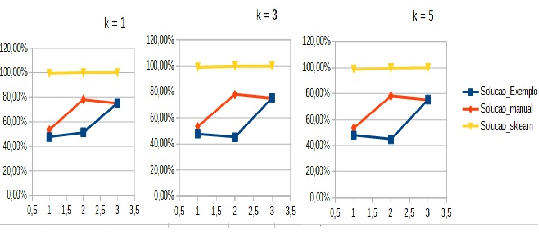
\includegraphics{figure 2}

\vspace{1.0cm}


Primeiro, analisando os resultados, podemos observar que a solução implementada com o algoritmo nativo do Sklearn foi de longe a mais eficiente entre os 3 modelos propostos, tanto do ponto de vista computacional, quanto no ajuste do modelo. A solução sklearn executa a tarefa em menos de 20s enquanto as demais soluções levam em média 8 minutos.


\vspace{1.0cm}

Além disso, podemos ver no gráfico que a solução exemplo e a solução manual tiveram pouca elasticidade em relação ao hiperparâmetro k, tendo quase o mesmo nível de precisão para k=1,k=3 ou k=5. 

\vspace{1.0cm}


Por último, é preciso mostrar que a distância euclidiana só se mostrou mais eficiente quando temos um grande número de amostras para treinamento em relação as amostras para validação.

\vspace{1.0cm}


Referências

\vspace{1.0cm}


[1] - https://scikit-learn.org/stable/modules/generated/sklearn.neighbors.KNeighborsClassifier.html

\vspace{1.0cm}


[2] - Evaluation of Jensen-Shannon Distance over Sparse Data - Richard ConnorFranco Alberto CardilloRobert MossFausto Rabitti

\vspace{1.0cm}

[3] - https://en.wikipedia.org/wiki/Euclidean_distance


\end{document}